% Chapter 4

\chapter{Experiments and Results} % Main chapter title

\label{Chapter4} % For referencing the chapter elsewhere, use \ref{Chapter4}

%----------------------------------------------------------------------------------------

This chapter reports every experiment in the order in which it was carried out. Each section states its purpose, set-up, result and the decision it led to; a one-page catalogue is in Appendix~\ref{AppendixA}. Percentages are changes in total rotation relative to the control named in the text; \emph{negative is better}. Results from the reduced protocols are exploratory (few runs, one instance per size, uncorrected $p$-values) and are labelled so.

%----------------------------------------------------------------------------------------

\section{Reproduction of ES-TRMP}\label{sec:exp-repro}

\textbf{Purpose.} Establish that the rebuilt code base reproduces the published algorithm, so that the published rows can serve as the baseline. \textbf{Set-up.} The original C source was rebuilt and run with 20 runs per instance on all 31 instances with $n\le100$, on \texttt{dirn200m120r150s06i00} ($n=198$) and on \texttt{dirn400m240r150s06i00} ($n=400$), and the new driver (baseline mode) was run on the same instances. \textbf{Result.} For all 33 instances the best, mean, standard deviation and the mean and standard deviation of the best-found iteration equal the reference results exactly (Table~\ref{tab:repro}). \textbf{Decision.} The published rows are used as the baseline for the 60-instance study; a same-session baseline is added later (Section~\ref{sec:exp-paired}) to remove any dependence on them.

\begin{table}[htbp]
\centering
\caption{Examples of exact reproduction (best / mean / SD over 20 runs, radians).}
\label{tab:repro}
\small
\begin{tabular}{lcccc}
\toprule
\textbf{Instance} & $n$ & \textbf{Best} & \textbf{Mean} & \textbf{SD}\\
\midrule
dirn050m030r150s03i00 & 18 & 97.458 & 97.458 & 0.000\\
dirn200m120r150s06i00 & 198 & 2198.577 & 2224.518 & 13.914\\
dirn400m240r150s06i00 & 400 & 4349.337 & 4373.350 & 17.225\\
\bottomrule
\end{tabular}
\end{table}

%----------------------------------------------------------------------------------------

\section{Diagnostic: Fixed Destruction Size}\label{sec:exp-diag}

\textbf{Purpose.} Before building a learner, find out whether the destruction size $\kappa$ influences solution quality at all; if offspring are nearly always identical in cost to the parent, or all $\kappa$ behave alike, no controller can help. \textbf{Set-up.} Baseline ES-TRMP with $\kappa\in\{2,4,6,8\}$ (uniform destroy, shuffle unchanged), paired seeds, on three instances: $n=100$ (\texttt{dirn100m060r150s06i03}, 10 runs), $n=198$ (\texttt{dirn200m120r150s06i00}, 10 runs) and $n=400$ (\texttt{dirn400m240r150s06i00}, 3 runs). The go/no-go rule was written before the results were inspected: no-go if more than 95\% of offspring tie the parent \emph{and} more than 99\% lie within $0.1\%$ of it for every $\kappa$; go if some $\kappa$ differs from $\kappa=4$ by at least $0.3\%$, consistently in sign across runs, on an instance with $n\ge198$, or if the ranking of $\kappa$ by gain per evaluation changes between budget phases.

\textbf{Result: offspring.} Table~\ref{tab:diag} and Figure~\ref{fig:outcomes} show that most offspring have exactly the parent's cost (82--99\%), that larger $\kappa$ converts ties mostly into \emph{worse} offspring (from $0.2$--$0.6\%$ at $\kappa=2$ up to $5$--$18\%$ at $\kappa=8$) while the share of \emph{better} offspring stays between about 0.4\% and 3\%, and that the evaluations per mutation grow in proportion to $\kappa$.

\begin{table}[htbp]
\centering
\caption{Mid-run (iterations 1000--3000) fate of offspring relative to the parent, uniform destroy. Evaluations per mutation (Eval/mut.) grow linearly with $\kappa$.}
\label{tab:diag}
\small
\begin{tabular}{llrrrrr}
\toprule
\textbf{Instance} & $\kappa$ & \textbf{Tie \%} & \textbf{Better \%} & \textbf{Worse \%} & \textbf{Eval/mut.}\\
\midrule
\multirow{3}{*}{$n=100$ (10 runs)} & 2 & 99.0 & 0.4 & 0.6 & 199\\
 & 4 & 95.4 & 0.5 & 4.0 & 394\\
 & 8 & 81.6 & 0.7 & 17.8 & 772\\
\midrule
\multirow{3}{*}{$n=198$ (10 runs)} & 2 & 98.4 & 1.1 & 0.5 & 395\\
 & 4 & 95.9 & 1.4 & 2.7 & 786\\
 & 8 & 87.4 & 1.4 & 11.1 & 1556\\
\midrule
\multirow{3}{*}{$n=400$ (3 runs)} & 2 & 96.5 & 3.3 & 0.2 & 799\\
 & 4 & 97.4 & 1.8 & 0.9 & 1594\\
 & 8 & 92.1 & 2.8 & 5.1 & 3172\\
\bottomrule
\end{tabular}
\end{table}

\begin{figure}[htbp]
\centering
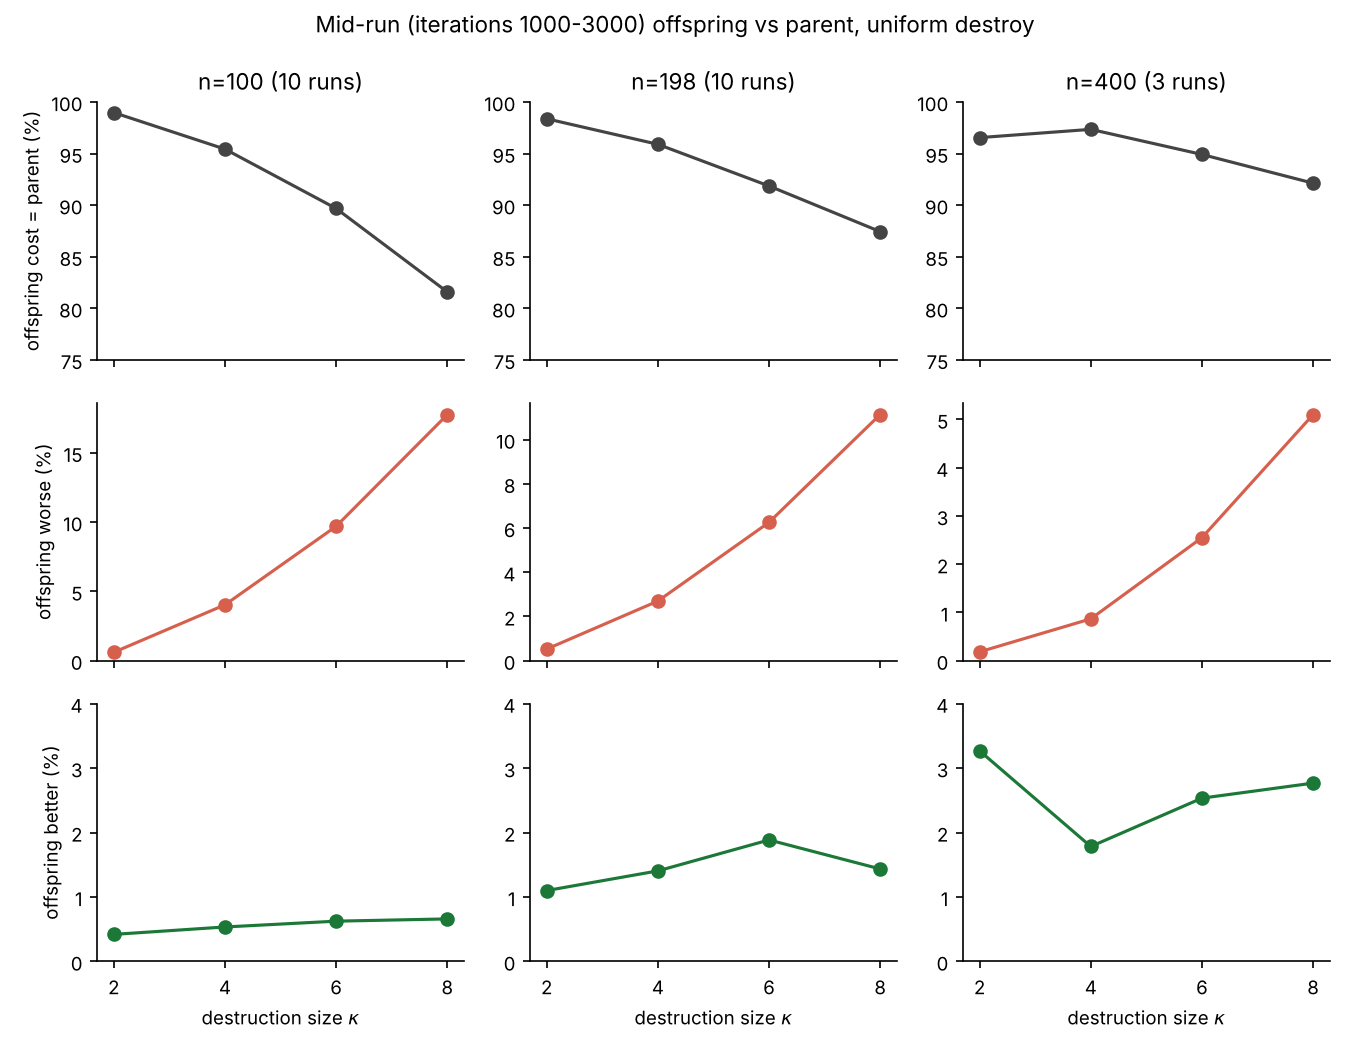
\includegraphics[width=0.92\textwidth]{Figures/fig1_outcomes_vs_kappa.png}
\caption{Mid-run offspring versus parent as the destruction size $\kappa$ grows (uniform destroy): ties fall, worse offspring rise sharply, better offspring barely change.}
\label{fig:outcomes}
\end{figure}

\textbf{Result: equal-budget quality.} Table~\ref{tab:diag-budget} compares best-so-far cost at equal evaluations. At $n=198$ with 10 runs every $\kappa$ ends within $0.08\%$ of $\kappa=4$ (all $p>0.8$); early in the run $\kappa=6$ is significantly \emph{worse} ($+0.47\%$ at 25\% of the budget, $p=0.027$; $+0.54\%$ at 50\%, $p=0.014$). At $n=100$, $\kappa=6$ and $\kappa=8$ are about $0.6\%$ better but not significantly. At $n=400$ with three runs $\kappa=2$ looked $0.36\%$ better in 3 of 3 runs but $0.43\%$ \emph{worse} at 25\% of the budget; with 10 paired runs (Section~\ref{sec:exp-policies}) $\kappa=2$ versus $\kappa=4$ is $+0.05\%$ ($p=0.77$), so the earlier figure was noise. Figure~\ref{fig:budgetcurve} shows the curves.

\begin{table}[htbp]
\centering
\caption{Equal-evaluation best-so-far at 100\% of the common budget, relative to $\kappa=4$ (negative is better); wins/losses are runs better/worse than $\kappa=4$.}
\label{tab:diag-budget}
\small
\begin{tabular}{lcccc}
\toprule
\textbf{Instance} & $\kappa=2$ & $\kappa=6$ & $\kappa=8$ & \textbf{runs}\\
\midrule
$n=100$ & $-0.17\%$ (5/5, $p=0.92$) & $-0.63\%$ (6/4, $p=0.38$) & $-0.56\%$ (7/3, $p=0.28$) & 10\\
$n=198$ & $-0.00\%$ (5/5, $p=0.85$) & $+0.02\%$ (6/4, $p=0.92$) & $+0.08\%$ (5/5, $p=1.0$) & 10\\
$n=400$ & $-0.36\%$ (3/0) & $+0.44\%$ (1/2) & $-0.20\%$ (2/1) & 3\\
$n=400$ (extended) & $+0.05\%$ (4/6, $p=0.77$) & --- & --- & 10\\
\bottomrule
\end{tabular}
\end{table}

\begin{figure}[htbp]
\centering
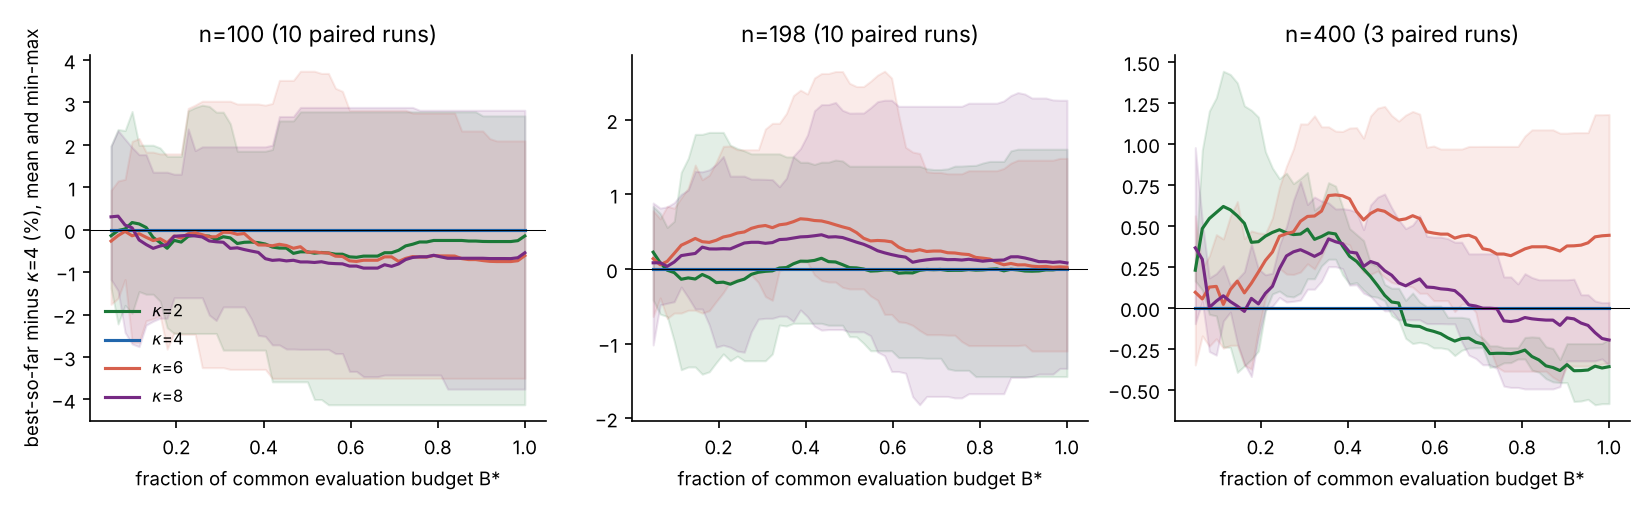
\includegraphics[width=\textwidth]{Figures/fig3_equal_budget_best.png}
\caption{Best-so-far minus the $\kappa=4$ value against the fraction of the common evaluation budget (paired runs; band = min--max). No $\kappa$ is reliably better than $\kappa=4$ at the end of the budget.}
\label{fig:budgetcurve}
\end{figure}

\textbf{Result: gain per evaluation.} The strict improvement of the incumbent per 1000 evaluations is largest for $\kappa=2$ in every budget quarter on all three instances (Figure~\ref{fig:gain}); because $\kappa=2$ is cheaper per mutation it makes more attempts per unit of budget. This does not translate into a better final solution, since all settings converge to the same neighbourhood.

\begin{figure}[htbp]
\centering
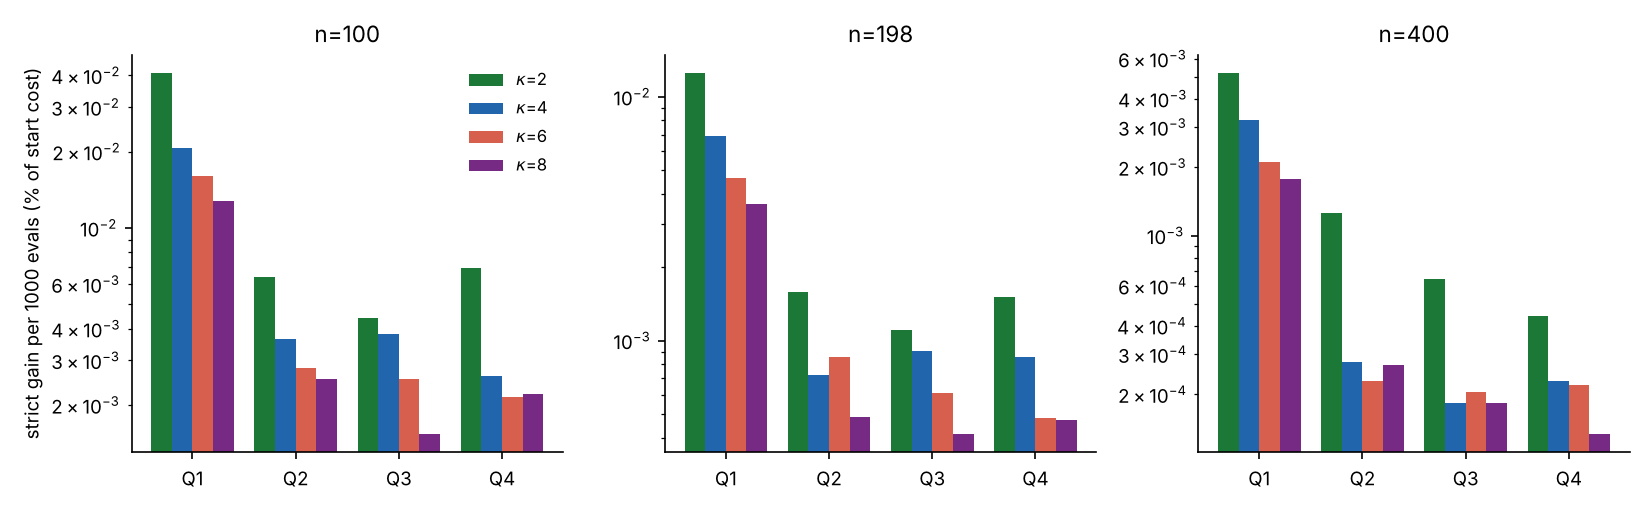
\includegraphics[width=\textwidth]{Figures/fig4_gain_per_1000_evals.png}
\caption{Strict incumbent improvement per 1000 evaluations by budget quarter (log scale; 10, 10 and 3 runs).}
\label{fig:gain}
\end{figure}

\textbf{Decision.} The no-go clause was not triggered ($\kappa=8$ has only 82--92\% ties), the \emph{go} condition (a) was met only technically at $n=400$ with three runs (the smallest attainable $p$ is $0.25$) and fails at $n=198$ with ten, and condition (b) fails because $\kappa=2$ ranks first in every quarter. The diagnostic was therefore read as inconclusive-to-negative for $\kappa$: do not start a learner on $\kappa$ alone without further evidence, and test selection policies cheaply first.

\paragraph{How many tied offspring are true no-operations?} An extra measurement (3 runs per cell, $n=100$ and $n=198$) separates ties into the \emph{identical permutation} (a true no-operation) and a \emph{different permutation of equal cost} (a plateau move that the algorithm accepts). At $\kappa=4$ only $3.9\%$ ($n=100$) and $16.4\%$ ($n=198$) of the mutations return the identical permutation; plateau moves are $91.2\%$ and $79.1\%$. The share of the evaluation budget spent on true no-operations is about $4\%$ and $16\%$ at $\kappa=4$, and $17$--$18\%$ ($n=100$) and $40$--$42\%$ ($n=198$) at $\kappa=2$ (Figure~\ref{fig:noop}). An earlier statement that \enquote{most of the budget is wasted on no-operations} was therefore too strong and was corrected.

\begin{figure}[htbp]
\centering
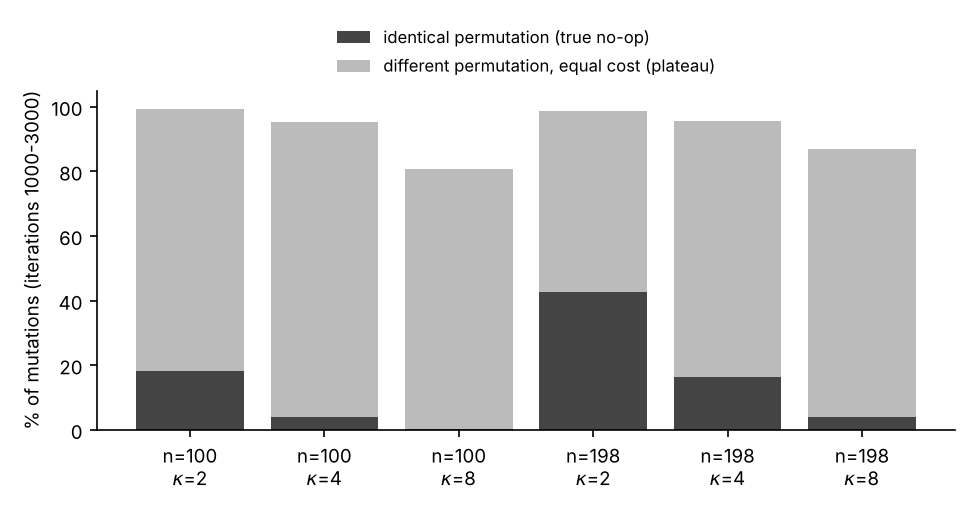
\includegraphics[width=0.85\textwidth]{Figures/fig5_noop_decomposition.png}
\caption{Tied offspring split into identical permutation (true no-op) and equal-cost different permutation (plateau move), iterations 1000--3000.}
\label{fig:noop}
\end{figure}

%----------------------------------------------------------------------------------------

\section{Reinforcement-Learning Controller for $\kappa$}\label{sec:exp-rl}

\textbf{Purpose.} Answer RQ1 directly: does a learned controller for $\kappa$ beat both the paper's fixed $\kappa=4$ and non-learning controls? \textbf{Set-up.} The controller of Section~\ref{sec:rlform} (differential and discounted variants) and the two controls were run on the three instances of Section~\ref{sec:exp-diag}, with 10, 10 and 3 paired runs, at the evaluation budget of the baseline run of the same index (parity within $0.098\%$). This is the \emph{reduced} protocol.

\textbf{Result.} Table~\ref{tab:rl} and Figure~\ref{fig:rlcontrols} give the outcome. Compared with the paper's $\kappa=4$, the differential controller is $-0.47\%$ ($n=100$), $-0.15\%$ ($n=198$) and $-0.25\%$ ($n=400$), none significant. The controls achieve the same: fixed $\kappa=2$ is $-0.44\%$, $-0.01\%$ and $-0.74\%$, random $\kappa$ is $-0.49\%$ and $+0.13\%$. Against fixed $\kappa=2$, the differential controller gains $-0.03\%$ ($p=0.56$) at $n=100$ and $-0.14\%$ ($p=0.63$) at $n=198$, and is $0.49\%$ \emph{worse} at $n=400$ (3 runs). The discounted variant is nominally the best RL arm at $n=100$ ($-1.10\%$, $p=0.027$ against $\kappa=4$) but is not significantly better than fixed $\kappa=2$ ($p=0.19$) or random $\kappa$ ($p=0.084$), and it gives only $-0.05\%$ at $n=198$.

\begin{table}[htbp]
\centering
\caption{Reduced-protocol RL results: best-so-far at 100\% of the equal budget, relative to uniform $\kappa=4$ (negative is better), and, in the last column, the RL gain over the fixed-$\kappa=2$ control. \texttt{block} (Section~\ref{sec:exp-policies}) is shown for reference.}
\label{tab:rl}
\small
\begin{tabular}{llrrl}
\toprule
\textbf{Instance} & \textbf{Method} & \textbf{vs $\kappa=4$} & $p$ & \textbf{RL vs fixed $\kappa=2$}\\
\midrule
\multirow{5}{*}{$n=100$ (10)} & fixed $\kappa=2$ & $-0.44\%$ & 0.63 & \\
 & random $\kappa$ & $-0.49\%$ & 0.63 & \\
 & RL differential & $-0.47\%$ & 0.63 & $-0.03\%$ ($p=0.56$)\\
 & RL discounted $\gamma=0.9$ & $-1.10\%$ & 0.027 & $-0.66\%$ ($p=0.19$)\\
 & \texttt{block} (no learning) & $-0.97\%$ & 0.084 & \\
\midrule
\multirow{5}{*}{$n=198$ (10)} & fixed $\kappa=2$ & $-0.01\%$ & 0.92 & \\
 & random $\kappa$ & $+0.13\%$ & 0.63 & \\
 & RL differential & $-0.15\%$ & 0.13 & $-0.14\%$ ($p=0.63$)\\
 & RL discounted $\gamma=0.9$ & $-0.05\%$ & 0.63 & $-0.05\%$ ($p=0.85$)\\
 & \texttt{block} (no learning) & $-1.79\%$ & 0.002 & \\
\midrule
\multirow{3}{*}{$n=400$ (3; \texttt{block} 5)} & fixed $\kappa=2$ & $-0.74\%$ & 0.25 (min.) & \\
 & RL differential & $-0.25\%$ & 0.75 & $+0.49\%$ (worse)\\
 & \texttt{block} (no learning) & $-2.66\%$ & 0.0625 (min.) & \\
\bottomrule
\end{tabular}
\end{table}

\begin{figure}[htbp]
\centering
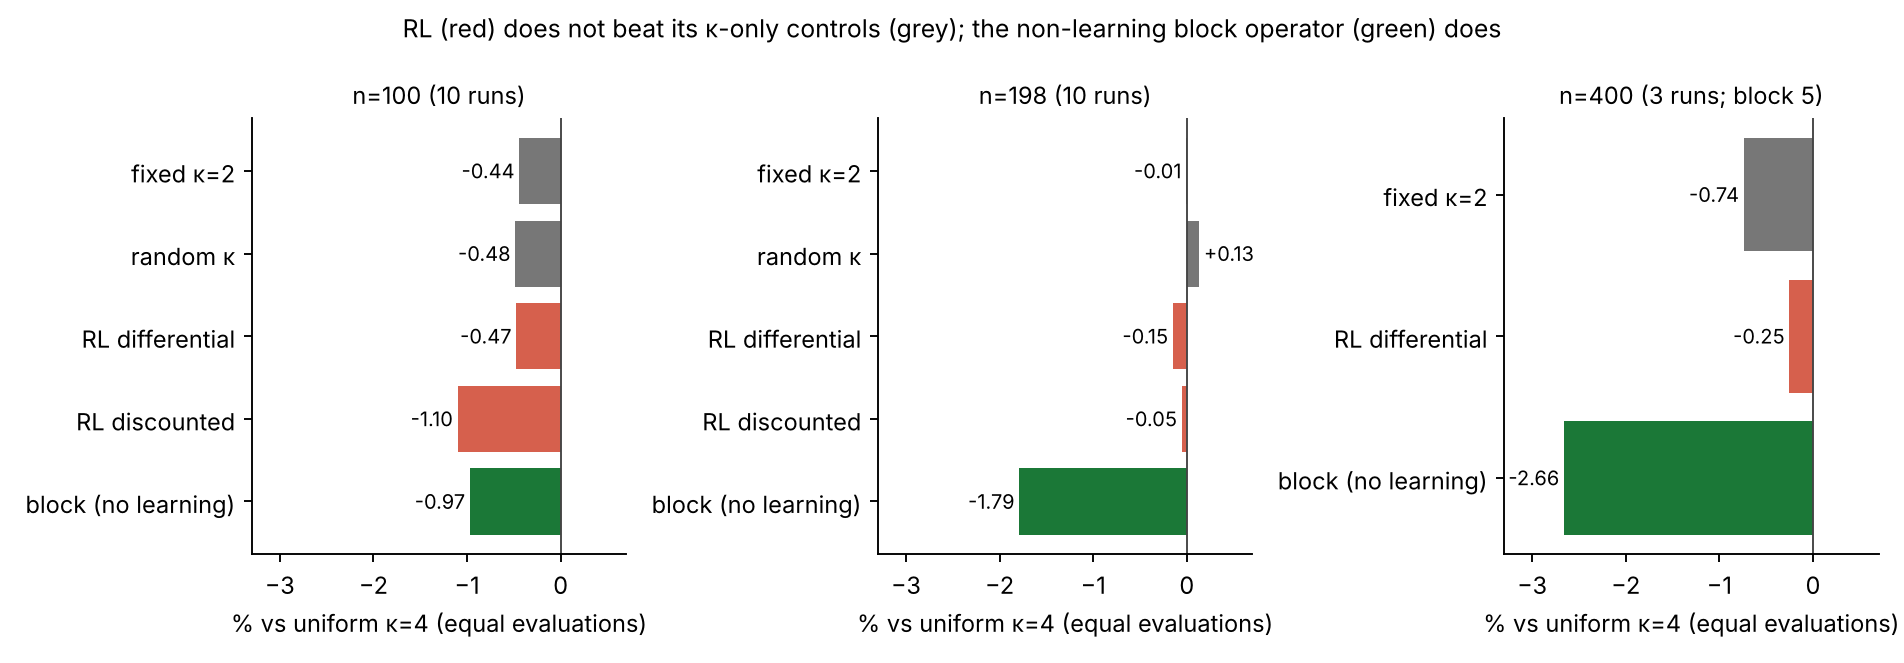
\includegraphics[width=\textwidth]{Figures/fig7_rl_vs_controls.png}
\caption{RL (red) against its $\kappa$-only controls (grey) and the non-learning \texttt{block} operator (green), same instance per panel, equal evaluations, percentage relative to uniform $\kappa=4$.}
\label{fig:rlcontrols}
\end{figure}

\textbf{Learned behaviour.} In every visited (stagnation $\times$ budget-quarter) cell the greedy action of the differential and the discounted controller is $\kappa=2$ at $n=100$, $198$ and $400$ (the one exception, the second budget quarter of the third stagnation bin at $n=100$, has $\kappa=4$ as its majority choice, with only 5 of 10 runs agreeing). The share of $\kappa=2$ choices at $n=198$ rises from 53\% to 67\% over the budget quarters; the remaining choices are largely $\varepsilon$-exploration. The within-state spread of $Q$ is small (median $0.035$ at $n=198$) and only $4.7\%$ of the rewards are non-zero ($2.7\%$ positive). The reward-rate estimate $\bar R$ stays finite after the time-unit fix but changes sign 26--72 times per run: its mean is about $10^{-2}$ in the first budget quarter at $n=198$ and about zero or slightly negative afterwards, i.e.\ the average reward rate is near zero, so the $-\bar R\tau$ term has little structure to work with. The learner's own cost (selection and update) is $0.003$--$0.008$\,s per run, below $0.01\%$ of the run time. Because $\kappa=2$ is cheaper, the controller performed 5069, 4861 and 4555 iterations in the budget in which the baseline performed 4000.

\textbf{Decision.} The controller learns a constant policy and does not beat its controls; its small advantages over $\kappa=4$ are explained by cost per mutation. Learning $\kappa$ was dropped as a method. The learner was kept as infrastructure and as a negative result. The scope of this result is limited to the reduced protocol, online learning, $\kappa$ as the only action and uniform destruction (Section~\ref{sec:discussion-limits}).

%----------------------------------------------------------------------------------------

\section{Destroy-Selection Policies}\label{sec:exp-policies}

\textbf{Purpose.} If $\kappa$ is not the lever, which groups are removed might be. \textbf{Set-up.} The policies of Section~\ref{sec:policies} were compared with uniform destruction at $\kappa=4$, paired, at equal evaluations, on the same three instances (10, 10 and 5 runs). The uniform policy was checked to be bit-identical to the baseline.

\textbf{Result.} Table~\ref{tab:policies} shows that \texttt{cost-greedy} gives no gain at any size, \texttt{history-aware} gives no effect at $n\le198$ and $-0.29\%$ at $n=400$ (5 of 5 runs, $p=0.0625$, after being slightly worse at 25--50\% of the budget), whereas \texttt{block} is better at every size: $-0.97\%$ ($n=100$, 8 of 10 runs), $-1.79\%$ ($n=198$, 10 of 10 runs, $p=0.002$) and $-2.66\%$ ($n=400$, 5 of 5 runs). At $n=400$ the \texttt{block} mean over the five runs (4257.5) is below the published mean (4373.35), while the uniform control over the same five runs gives 4374.0, in line with the published mean. The extra experiment of $\kappa=2$ versus $\kappa=4$ at $n=400$ with ten paired runs is also reported here: $+0.18\%$, $+0.09\%$, $+0.05\%$ at 25, 50 and 100\% of the budget ($p=0.13$, $0.56$, $0.77$).

\begin{table}[htbp]
\centering
\caption{Destroy-selection policies at $\kappa=4$: percentage of mutations that are ties and that are worse than the parent (mid-run), and equal-evaluation best at 100\% of the budget relative to uniform (wins/losses of the policy; $p$ Wilcoxon). With 5 runs the smallest attainable $p$ is 0.0625.}
\label{tab:policies}
\small
\begin{tabular}{llrrl}
\toprule
\textbf{Instance} & \textbf{Policy} & \textbf{Tie \%} & \textbf{Worse \%} & \textbf{100\% budget}\\
\midrule
\multirow{4}{*}{$n=100$ (10)} & uniform & 95.4 & 4.0 & ---\\
 & \texttt{cost-greedy} & 94.7 & 4.7 & $+0.31\%$ (5/5, $p=0.70$)\\
 & \texttt{history-aware} & 93.7 & 5.6 & $-0.04\%$ (4/6, $p=1.0$)\\
 & \texttt{block} & 89.3 & 10.1 & $-0.97\%$ (8/2, $p=0.084$)\\
\midrule
\multirow{4}{*}{$n=198$ (10)} & uniform & 95.9 & 2.7 & ---\\
 & \texttt{cost-greedy} & 94.4 & 4.0 & $+0.13\%$ (5/5, $p=0.63$)\\
 & \texttt{history-aware} & 94.0 & 4.6 & $+0.15\%$ (5/5, $p=0.63$)\\
 & \texttt{block} & 74.5 & 24.1 & $-1.79\%$ (10/0, $p=0.002$)\\
\midrule
\multirow{4}{*}{$n=400$ (5)} & uniform & 97.0 & 0.9 & ---\\
 & \texttt{cost-greedy} & 95.8 & 1.9 & $+0.22\%$ (2/3, $p=0.63$)\\
 & \texttt{history-aware} & 95.5 & 2.0 & $-0.29\%$ (5/0, $p=0.0625$)\\
 & \texttt{block} & 83.8 & 13.3 & $-2.66\%$ (5/0, $p=0.0625$)\\
\bottomrule
\end{tabular}
\end{table}

\textbf{Decision.} \texttt{block} was adopted for validation; \texttt{cost-greedy} was dropped (no gain); \texttt{history-aware}, the policy motivated by the multi-predecessor structure, was dropped as unproven (it would need at least ten runs at $n=400$ before any claim).

%----------------------------------------------------------------------------------------

\section{Does \texttt{block} Generalise?}\label{sec:exp-validate}

\textbf{Purpose.} Establish whether the \texttt{block} gain holds beyond the single instance on which it was found. \textbf{Set-up.} Three different instances per size class, covering the three apertures, were compared against uniform at $\kappa=4$ (10 runs at $n\approx100,200$; 5 runs at $n=400$). The rule was pre-registered: \texttt{block} \emph{generalises} for a size if it is better at 100\% budget on at least two of three instances, none is significantly worse, and the mean per-instance gain is at least $0.5\%$.

\textbf{Result.} Table~\ref{tab:validate} shows that at $n\approx200$ \texttt{block} wins on all three instances ($-1.18\%$ to $-2.39\%$, mean $-1.95\%$, each $p\le0.004$) and at $n=400$ on all three ($-2.43\%$ to $-2.82\%$, mean $-2.68\%$; every one of the 15 paired runs favours \texttt{block}). At $n\approx100$ it does not generalise: better on one of three instances, mean $-0.04\%$; the early advantage seen on one instance ($-0.63\%$ at 25\% of the budget, $p=0.049$) disappears by the end of the budget. The rule is met at $n\approx200$ and $n=400$ and not at $n\approx100$.

\begin{table}[htbp]
\centering
\caption{\texttt{block} versus uniform at $\kappa=4$, 100\% of the equal budget (negative is better).}
\label{tab:validate}
\small
\begin{tabular}{llrrrr}
\toprule
\textbf{Size} & \textbf{Instance (aperture)} & \textbf{Runs} & \textbf{Change} & \textbf{W/L} & $p$\\
\midrule
$n\approx100$ & s03i03 ($n=94$) & 10 & $-0.46\%$ & 6/4 & 0.23\\
 & s04i02 ($n=99$) & 10 & $+0.10\%$ & 4/6 & 0.77\\
 & s06i04 ($n=96$) & 10 & $+0.24\%$ & 4/6 & 0.70\\
\midrule
$n\approx200$ & s03i03 ($n=200$) & 10 & $-1.04\%$ & 9/1 & 0.004\\
 & s04i01 ($n=200$) & 10 & $-2.41\%$ & 10/0 & 0.002\\
 & s06i01 ($n=200$) & 10 & $-2.40\%$ & 9/1 & 0.004\\
\midrule
$n=400$ & s03i00 & 5 & $-2.43\%$ & 5/0 & 0.0625\\
 & s04i00 & 5 & $-2.79\%$ & 5/0 & 0.0625\\
 & s06i01 & 5 & $-2.82\%$ & 5/0 & 0.0625\\
\bottomrule
\end{tabular}
\end{table}

\textbf{Decision.} \texttt{block} is real and size-dependent: adopted for $n\gtrsim200$; neutral at $n\approx100$.

%----------------------------------------------------------------------------------------

\section{Destruction Size for \texttt{block}}\label{sec:exp-bk}

\textbf{Purpose.} Check whether the gain depends on $\kappa=4$, and whether it survives against the best \emph{uniform} $\kappa$. \textbf{Set-up.} \texttt{block} with $\kappa\in\{2,4,6,8,12\}$ and uniform with $\kappa\in\{2,4\}$ on $n=198$ (10 runs) and \texttt{dirn400m240r150s04i00} (5 runs), compared at the smallest common evaluation total.

\textbf{Result.} Table~\ref{tab:bk} gives the values relative to uniform $\kappa=4$. At $n=198$, \texttt{block} with $\kappa\in\{4,6,8,12\}$ is equivalent (within $0.05\%$), $\kappa=2$ is clearly worse ($+1.38\%$ relative to \texttt{block} $\kappa=4$, $p=0.004$). At $n=400$ there is a non-significant trend towards larger $\kappa$ ($\kappa=12$: $-0.77\%$ relative to \texttt{block} $\kappa=4$, 4 wins and 1 loss, $p=0.44$). The gain survives the best uniform $\kappa$: \texttt{block} $\kappa=4$ beats uniform $\kappa=2$ by $-1.87\%$ (10/0, $p=0.002$) at $n=198$ and $-2.60\%$ (5/0) at $n=400$. Large $\kappa$ values are judged after only about 17--34\% of their own run, because the common budget is set by the cheapest arm.

\begin{table}[htbp]
\centering
\caption{Block $\kappa$ sweep, equal evaluations at 100\% of the common budget, relative to uniform $\kappa=4$.}
\label{tab:bk}
\small
\begin{tabular}{lcccccc}
\toprule
 & \textbf{unif.\ 2} & \textbf{blk 2} & \textbf{blk 4} & \textbf{blk 6} & \textbf{blk 8} & \textbf{blk 12}\\
\midrule
$n=198$ (10 runs) & $-0.00\%$ & $-0.52\%$ & $-1.87\%$ & $-1.83\%$ & $-1.82\%$ & $-1.86\%$\\
$n=400$ (5 runs) & $-0.24\%$ & $-1.74\%$ & $-2.83\%$ & $-3.17\%$ & $-3.14\%$ & $-3.58\%$\\
\bottomrule
\end{tabular}
\end{table}

\textbf{Decision.} The paper's $\kappa=4$ is retained for the headline results (no tuning on the evaluation data); larger $\kappa$ for \texttt{block} at $n=400$ is a lead for future work.

%----------------------------------------------------------------------------------------

\section{Why Does \texttt{block} Work? Mechanism Controls}\label{sec:exp-mech}

\textbf{Purpose.} Answer RQ2: separate the ingredients of \texttt{block}. It differs from uniform in two ways at once, \emph{which} set is removed (adjacent groups) and the \emph{order} in which they are re-inserted (ascending positions instead of random draw order). \textbf{Set-up.} The control variants of Section~\ref{sec:policies} on $n=100$ and $n=198$ (10 paired runs), at $\kappa=4$, equal evaluations; the decision rules were pre-registered.

\textbf{Result.} Table~\ref{tab:mech} shows that contiguity of the removed set is the active ingredient: \texttt{block-rord} (contiguous, random re-insertion order) is $-1.61\%$ at $n=198$ (10/0, $p=0.002$), and beats \texttt{uniform-sorted} (uniform selection, ascending order) by $-1.71\%$ (10/0, $p=0.002$). Re-insertion order does not matter (\texttt{uniform-sorted} $+0.10\%$; \texttt{block} versus \texttt{block-rord} $-0.18\%$, $p=0.32$), and neither does the edge behaviour of the start position (\texttt{wrap} $-1.56\%$; \texttt{wrap} versus \texttt{block} $+0.24\%$, $p=0.32$). The direction at $n=100$ is the same but weaker and mostly non-significant.

\begin{table}[htbp]
\centering
\caption{Mechanism controls at $\kappa=4$, equal evaluations at 100\% of the budget, relative to uniform (10 paired runs).}
\label{tab:mech}
\small
\begin{tabular}{lcc}
\toprule
\textbf{Arm} & $n=100$ & $n=198$\\
\midrule
\texttt{uniform-sorted} & $-0.60\%$ (5/5, $p=0.23$) & $+0.10\%$ (5/5, $p=0.49$)\\
\texttt{block} & $-0.97\%$ (8/2, $p=0.084$) & $-1.79\%$ (10/0, $p=0.002$)\\
\texttt{block-rord} & $-1.63\%$ (8/2, $p=0.064$) & $-1.61\%$ (10/0, $p=0.002$)\\
\texttt{wrap} & $-0.70\%$ (6/4, $p=0.49$) & $-1.56\%$ (10/0, $p=0.002$)\\
\bottomrule
\end{tabular}
\end{table}

\textbf{Offspring descriptors.} At $n=198$ (iterations 1000--3000) contiguous removal produces many more \emph{worse} offspring ($24$--$39\%$ versus $2.7\%$ for uniform) and fewer plateau moves, while the share of \emph{better} offspring is essentially unchanged ($1.3$--$1.5\%$). The removed set of \texttt{block} is not more costly than a uniform draw (mean removed cost $43.9$ against $45.1$), so \texttt{block} is not acting as a \texttt{cost-greedy} proxy. Over the whole run, strict improvements occur about $14\%$ more often per mutation with \texttt{block} (333 against 291 per 10{,}000 mutations) with essentially the same size per success (mean relative gain $0.070\%$ against $0.067\%$), and the gap in best-so-far is already $-1.63\%$ after a quarter of the budget, $-1.88\%$ after half and $-1.79\%$ at the end. The mechanism claim is therefore limited to \emph{contiguity of the removed set}. The leading explanation, not tested here, is that adjacent groups share sensor-orientation history, so removing them together lets the greedy repair re-optimise them jointly, whereas widely separated removals behave like independent single-group re-insertions that an already-converged search rarely improves. A window-restricted random-subset control would separate adjacency from locality.

%----------------------------------------------------------------------------------------

\section{Mixed Operators}\label{sec:exp-mix}

\textbf{Purpose.} If neither operator dominates, a controller that chooses between them per mutation could add value. \textbf{Set-up.} \texttt{mix:}$p$ applies \texttt{block} with probability $p\in\{0.25,0.5,0.75\}$ and uniform otherwise, drawn from a private generator ($n=100$ and $n=198$, 10 runs). Rule: a mix \emph{beats} \texttt{block} if it is at least $0.3\%$ better on both sizes with $p<0.1$ at $n=198$.

\textbf{Result.} No mix beats \texttt{block}. At $n=198$, mean best falls monotonically as the block share rises: $2227.5$ (0\%), $2203.0$, $2202.2$, $2197.4$ and $2187.6$ (100\%), i.e.\ $-1.10\%$, $-1.13\%$, $-1.35\%$ and $-1.79\%$ relative to uniform, with every mix $0.44$--$0.67\%$ \emph{worse} than pure \texttt{block} (two of three $p<0.05$). The one mix that looked good at $n=100$ ($p=0.75$, $-0.83\%$ against \texttt{block}, $p=0.064$) does not replicate at $n=198$.

\textbf{Per-state evidence.} Splitting the strict-improvement rate by stagnation quartile and budget quarter shows that the only significant cells (low stagnation, first quarter) favour \texttt{block}; no cell significantly favours uniform. The pre-registered rule for a state-dependent preference (at least two significant cells of opposite sign) is not met at $n\le198$. Strict improvements are too rare in late and high-stagnation states to resolve any state dependence at this sample size. At $n=400$ (one instance, 5 runs, pure arms only) \texttt{block} is $-2.79\%$ (5 of 5 runs, $p=0.0625$) and appears better early and uniform better in the last quarter; this is a single-instance lead and is unconfirmed. Mixed operators at $n=400$ were not completed.

\textbf{Decision.} Mixing was dropped. A learner over $\{$uniform, \texttt{block}$\}$ was not built because pure \texttt{block} already dominates in every state that could be resolved.

%----------------------------------------------------------------------------------------

\section{Full-Protocol Results Against the Published ES-TRMP}\label{sec:exp-full}

\textbf{Purpose.} Answer RQ3 under the original protocol. \textbf{Set-up.} \texttt{block} with $\kappa=4$ and uniform shuffle, 4{,}000 iterations, 20 runs (seeds $1,\ldots,20$), on all 60 instances, compared with the published ES-TRMP rows. For each instance the change of the 20-run mean is computed; groups are compared with the Wilcoxon signed-rank test over instance means (instances with identical means excluded).

\textbf{Result.} Table~\ref{tab:full} and Figure~\ref{fig:full} summarise the outcome. On the 26 instances with $n\ge198$ the mean improves on \emph{all 26}, by $2.17\%$ on average (range $-1.18\%$ to $-3.07\%$; $p<0.0001$); on the 15 instances with $n=400$ the average is $-2.32\%$ (15 of 15). The gain grows with the instance size and is present for all three apertures (Table~\ref{tab:aperture}), largest for the hardest aperture ($\pi/3$). On the 21 instances with $n\le50$ the results are unchanged (7 better, 7 equal, 7 worse, mean $0.00\%$; the algorithm already converges there). Over all 60 instances the mean change is $-1.03\%$ (median $-0.51\%$; 45 better, 7 equal, 8 worse). The best solution found in 20 runs improves on all 26 instances with $n\ge198$ and on 37 of 60 instances overall (19 unchanged, 4 worse: $n=28$, $36$, $100$ and $145$). The eight instances with a marginally worse mean all have $n\le78$ and lose at most $0.52\%$.

\begin{table}[htbp]
\centering
\caption{Full-protocol change of the 20-run mean relative to the published ES-TRMP (negative is better).}
\label{tab:full}
\small
\begin{tabular}{lrrrr}
\toprule
\textbf{Instances} & \textbf{Count} & \textbf{Mean change} & \textbf{Better / equal / worse} & \textbf{Wilcoxon $p$}\\
\midrule
$n\le50$ & 21 & $0.00\%$ & 7 / 7 / 7 & 0.90\\
$50<n\le100$ & 10 & $-0.35\%$ & 9 / 0 / 1 & 0.0098\\
$100<n<200$ & 5 & $-1.13\%$ & 5 / 0 / 0 & ---\\
$n=200$ & 9 & $-1.97\%$ & 9 / 0 / 0 & 0.0039\\
$n=400$ & 15 & $-2.32\%$ & 15 / 0 / 0 & 0.0001\\
\textbf{$n\ge198$} & \textbf{26} & $\mathbf{-2.17\%}$ & \textbf{26 / 0 / 0} & $<0.0001$\\
All & 60 & $-1.03\%$ & 45 / 7 / 8 & $<0.0001$\\
\bottomrule
\end{tabular}
\end{table}

\begin{table}[htbp]
\centering
\caption{Full-protocol result for $n\ge198$ by sensing angle $\varphi$.}
\label{tab:aperture}
\small
\begin{tabular}{lrrrr}
\toprule
$\varphi$ & \textbf{Instances} & \textbf{Mean change} & \textbf{Better} & \textbf{Wilcoxon $p$}\\
\midrule
$2\pi/3$ & 7 & $-1.83\%$ & 7/7 & 0.0156\\
$\pi/2$ & 9 & $-2.12\%$ & 9/9 & 0.0039\\
$\pi/3$ & 10 & $-2.45\%$ & 10/10 & 0.0020\\
\bottomrule
\end{tabular}
\end{table}

\begin{figure}[htbp]
\centering
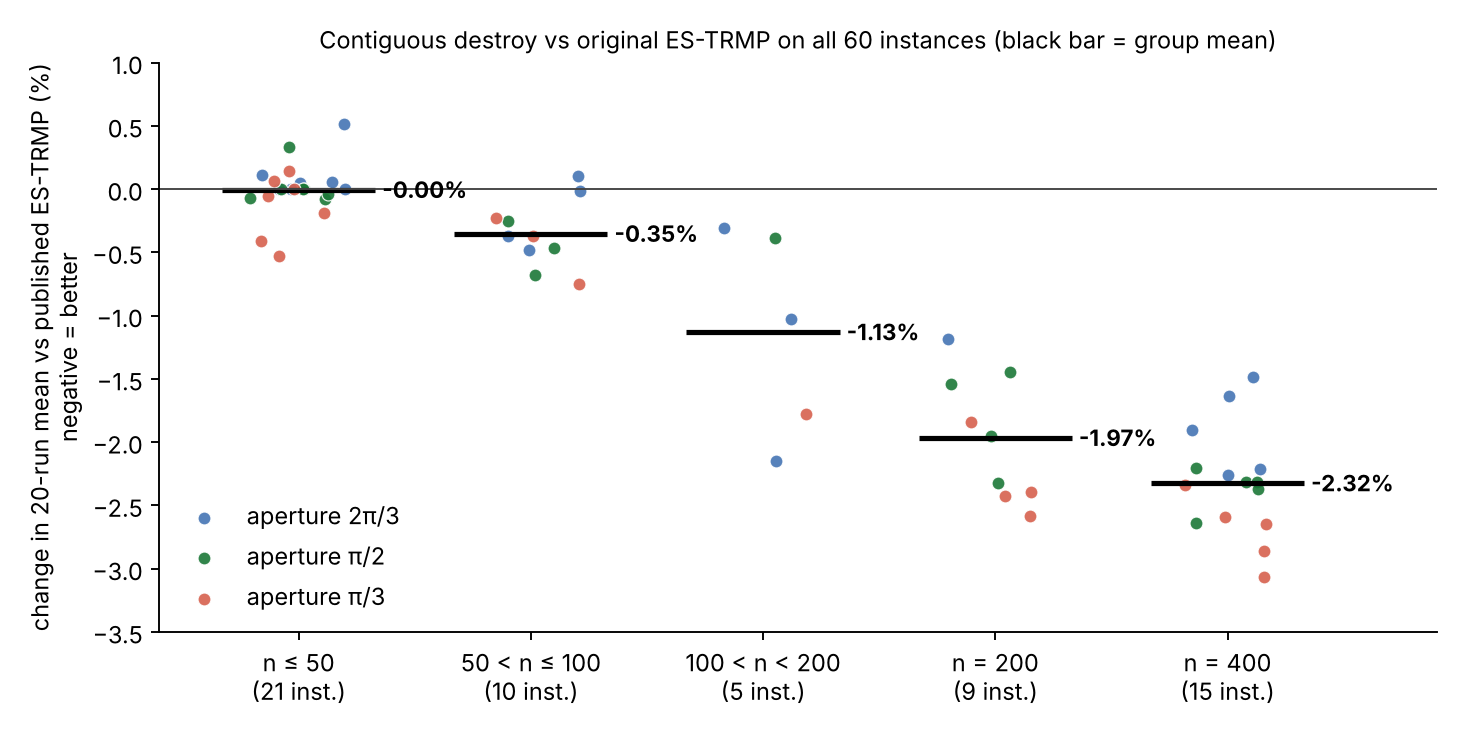
\includegraphics[width=\textwidth]{Figures/fig6_full_protocol.png}
\caption{Change in the 20-run mean solution cost per instance (negative is better than the published ES-TRMP), grouped by size; colours indicate the sensing angle and the black bar is the group mean.}
\label{fig:full}
\end{figure}

Table~\ref{tab:examples} gives examples in the paper's units (radians), together with the previous method's mean from the same paper for context. For \texttt{dirn400m240r150s06i00} the gain of $102.4$ equals about $26$ standard errors of the published mean (SD 17.2 over 20 runs). The per-instance results of all 60 instances are in Appendix~\ref{AppendixB}.

\begin{table}[htbp]
\centering
\caption{Example instances: mean total rotation (radians). GA-TRMP+LSB values are the previous method's published figures, quoted for context only; the GA was not re-run.}
\label{tab:examples}
\small
\begin{tabular}{lrrrrr}
\toprule
\textbf{Instance} & $n$ & \textbf{GA-TRMP+LSB} & \textbf{ES-TRMP} & \textbf{With block} & \textbf{Change}\\
\midrule
dirn200m120r150s06i00 & 198 & 2311.846 & 2224.518 & 2184.983 & $-1.78\%$\\
dirn400m240r150s06i00 & 400 & 4594.853 & 4373.350 & 4270.926 & $-2.34\%$\\
dirn400m240r150s06i01 & 400 & 4015.341 & 3801.517 & 3692.783 & $-2.86\%$\\
dirn400m240r150s06i02 & 400 & 4146.541 & 3920.388 & 3800.164 & $-3.07\%$\\
\bottomrule
\end{tabular}
\end{table}

\textbf{Variance and cost.} The run-to-run standard deviation is \emph{not} reduced: the median ratio of the standard deviation with \texttt{block} to that of ES-TRMP is $1.12$ at $n\ge198$ (the expectation in the design brief of a variance reduction is not supported; the gain is in the mean). The operator changes no repair work, so the candidate evaluations per mutation are identical (for example $6.57\times10^6$ against $6.53\times10^6$ per $n=400$ run, Section~\ref{sec:exp-paired}), and the full 60-instance, 20-run study used 22.1 CPU-hours.

%----------------------------------------------------------------------------------------

\section{Same-Session Paired Confirmation}\label{sec:exp-paired}

\textbf{Purpose.} The full-protocol comparison uses the published rows, which contain only per-instance means. To remove any dependence on them and to test per run, the \emph{original} algorithm was re-run in this session on a subset and paired with \texttt{block}, run by run. \textbf{Set-up.} Ten instances covering all apertures: $n=94,100$ (2 instances), $n=198,200,200,200$ (4 instances) and $n=400$ (4 instances), 20 paired runs each (same seeds and thus the same pre-processed start). \textbf{Validity check.} The same-session baseline mean equals the published mean on 10 of 10 instances.

\textbf{Result.} Table~\ref{tab:paired} lists the instances and Table~\ref{tab:pooled} the pooled results. At $n\ge198$ \texttt{block} is better in 157 of 160 paired runs, with a pooled mean change of $-2.18\%$ (95\% bootstrap interval $-2.50\%$ to $-1.81\%$); at $n=400$ in all 80 of 80. Paired effect sizes at $n\ge198$ are large ($|d_z|$ between 1.3 and 4.9). At $n\approx100$ the per-instance $p$ values ($0.048$ and $0.040$) do not survive Holm correction across the ten tests ($0.08$), so that size is only suggestive. The standard deviation ratio at $n\ge198$ is again about $1.09$. Per-run times are within $\pm15\%$ of the original (CPU seconds per run, measured with parallel jobs sharing the machine and therefore approximate): $n\approx200$: 45\,s original, 39\,s \texttt{block}; $n=400$: 238\,s and 254\,s.

\begin{table}[htbp]
\centering
\caption{Same-session paired comparison, 20 runs per instance (negative is better).}
\label{tab:paired}
\small
\begin{tabular}{lrrrrrr}
\toprule
\textbf{Instance} & $n$ & \textbf{Uniform} & \textbf{Block} & \textbf{Change} & \textbf{Better/worse} & $d_z$\\
\midrule
dirn100m060r150s03i03 & 94 & 305.439 & 303.957 & $-0.48\%$ & 13/7 & $-0.50$\\
dirn100m060r150s06i03 & 100 & 392.536 & 389.603 & $-0.73\%$ & 15/5 & $-0.49$\\
dirn200m120r150s06i00 & 198 & 2224.518 & 2184.983 & $-1.78\%$ & 20/0 & $-2.29$\\
dirn200m120r150s03i03 & 200 & 749.745 & 740.870 & $-1.18\%$ & 18/2 & $-1.30$\\
dirn200m120r150s04i01 & 200 & 1397.124 & 1364.673 & $-2.32\%$ & 20/0 & $-2.25$\\
dirn200m120r150s06i01 & 200 & 1340.500 & 1308.422 & $-2.39\%$ & 19/1 & $-2.39$\\
dirn400m240r150s03i00 & 400 & 2569.235 & 2511.092 & $-2.26\%$ & 20/0 & $-3.61$\\
dirn400m240r150s04i00 & 400 & 3267.053 & 3191.441 & $-2.31\%$ & 20/0 & $-3.03$\\
dirn400m240r150s06i00 & 400 & 4373.350 & 4270.926 & $-2.34\%$ & 20/0 & $-4.87$\\
dirn400m240r150s06i01 & 400 & 3801.517 & 3692.783 & $-2.86\%$ & 20/0 & $-3.99$\\
\bottomrule
\end{tabular}
\end{table}

\begin{table}[htbp]
\centering
\caption{Pooled same-session results (cluster bootstrap over instances then runs).}
\label{tab:pooled}
\small
\begin{tabular}{lrrrr}
\toprule
\textbf{Group} & \textbf{Instances} & \textbf{Mean change} & \textbf{95\% CI} & \textbf{Runs better}\\
\midrule
$n\approx100$ & 2 & $-0.60\%$ & $[-1.06,-0.21]$ & 28 / 40\\
$n\approx200$ (198--200) & 4 & $-1.92\%$ & $[-2.39,-1.39]$ & 77 / 80\\
$n=400$ & 4 & $-2.44\%$ & $[-2.74,-2.20]$ & 80 / 80\\
\textbf{$n\ge198$} & \textbf{8} & $\mathbf{-2.18\%}$ & $\mathbf{[-2.50,-1.81]}$ & \textbf{157 / 160}\\
Whole subset & 10 & $-1.86\%$ & $[-2.33,-1.36]$ & 185 / 200\\
\bottomrule
\end{tabular}
\end{table}

\textbf{Decision.} The headline result stands under the paired design: \texttt{block} improves ES-TRMP by about $2\%$ at $n\ge198$.
